\documentclass{diplomka}
%\usepackage[cp1250]{inputenc}
\usepackage{listings}
\usepackage[utf8]{inputenc} 
\usepackage[czech]{babel}
\usepackage{ae}
\usepackage{fancyhdr}
\usepackage{float}
\usepackage{graphicx}
\usepackage{multirow}
\usepackage{color, colortbl}
\usepackage{enumitem}
\usepackage{array}
\usepackage{caption}
\usepackage{subcaption}

%\usepackage[pdftex]{graphicx}

\lstset{language=Java,keywordstyle=\color{blue}, commentstyle=\color{Green},stringstyle=\color{red},showstringspaces=false,breaklines=true,tabsize=3,basicstyle=\footnotesize}



\author{Martin Kadlec}
\title{Docházka a výkazy práce pro systém IMIS na platformě Android}
\titlet{}
\titlett{}
\university{Západočeská univerzita v Plzni}
\faculty{Fakulta aplikovaných věd}
\department{Katedra informatiky a výpočetní techniky}
\subject{Diplomová práce}
\town{Plzeň}
\begin{document}
\pagestyle{fancy}
\renewcommand{\chaptermark}[1]{\markboth{\textit{#1}}{}}
\renewcommand{\sectionmark}[1]{\markright{\textit{#1}}{}}
\cfoot{\thepage}
\lhead{\leftmark}
\rhead{\rightmark}
\maketitle
\chapter*{Prohlášení}
\thispagestyle{empty}
Prohlašuji, že jsem bakalářskou práci vypracoval samostatně a výhradně s~použitím citovaných pramenů.
\vskip 1.5em
V Plzni dne \today
\vskip 0.7em
\hskip 9cm Maxipes Fík
\chapter*{Abstract}
\thispagestyle{empty}
Text of abstract.
\pagestyle{empty}
\tableofcontents
\pagestyle{fancy}
\renewcommand{\chaptermark}[1]{\markboth{\textit{#1}}{}}
\renewcommand{\sectionmark}[1]{\markright{\textit{#1}}{}}
\cfoot{\thepage}
\lhead{\leftmark}
\rhead{\rightmark}
\parskip 1em

%\renewcommand{\chaptermark}[1]{\markboth{\textit{#1}}{}}
%\renewcommand{\sectionmark}[1]{\markright{\textit{#1}}{}}
\chapter{Úvod}

\chapter{Současný systém}
Integrovaný manažerský informační systém (IMIS) je součástí informačního systému Ramses ERP vyvinutého společností CCA Group a.s. Jedná se modulový ERP systém zabývající se oblastmi podnikových financí, kontrolováním nákladů, personalistikou a činnostmi podporující obchod. Společnost tento systém sama využívá pro svoje interní potřeby.

\section{Vybraná funkcionalita}
V této práci se zaměřuji na funkcionalitu z oblasti systému věnující se personalistice. Konktrétně se jedná o moduly pro zápis příchodů a odchodů na pracovistě a vykazování provedené práce. Jedná se o činnosti, které zaměstnanec provádí jako každodenní rutinu a zároveň jsou to činnosti s nejširší skupinou uživatelů v rámci podniku.
 
\subsection{Evidence docházky}
Docházkový systém slouží k evidenci docházky zaměstnanců, která se následně využívá k přípravě podkladů pro zpracování mzdové agendy.\\ \indent
Eviduje se každý příchod i odchod z pracoviště společně s účelem události. Účel události je důležitý, protože délka pracovní přestávky či odchod z pracoviště k lékaři jsou legislativně ošetřené záležitosti.\\ \indent Každá událost se zaznamenává s přesností na minuty. Časová osa s průběhem běžného pracovního dne je zobrazena na obr. \ref{obr:attn}.
\begin{figure}[H]
  \centering
  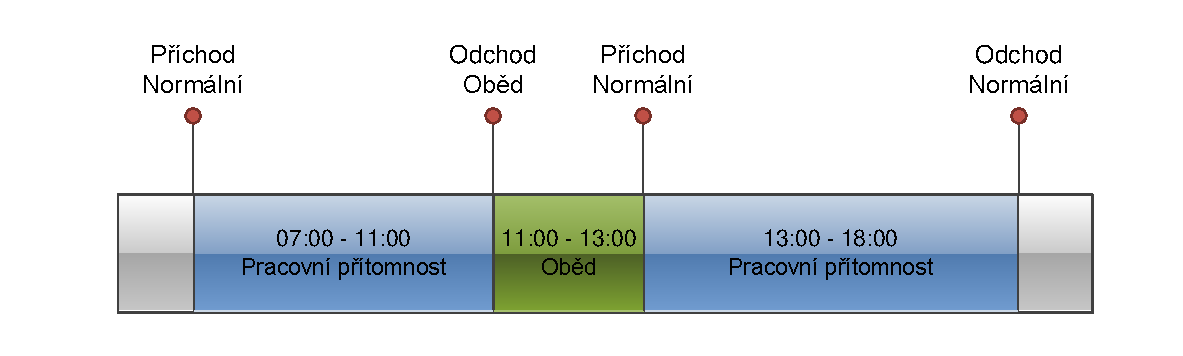
\includegraphics[scale=0.7]{visio/attnormal.pdf}
\caption{Časová osa běžného pracovního dne}
\label{obr:attn}
\end{figure}

Na obrázku \ref{obr:atts} je znázorněn pracovní den se služební cestou. Zaměstnanec nejprve zadá příchod do normální pracovní doby a s minutovým odstupem následuje služební odchod. Podobně musí zadat i návrat, nejprve zadá příchod do normální pracovní doby a s minutovým odstupem následuje normální odchod.
\begin{figure}[H]
  \centering
  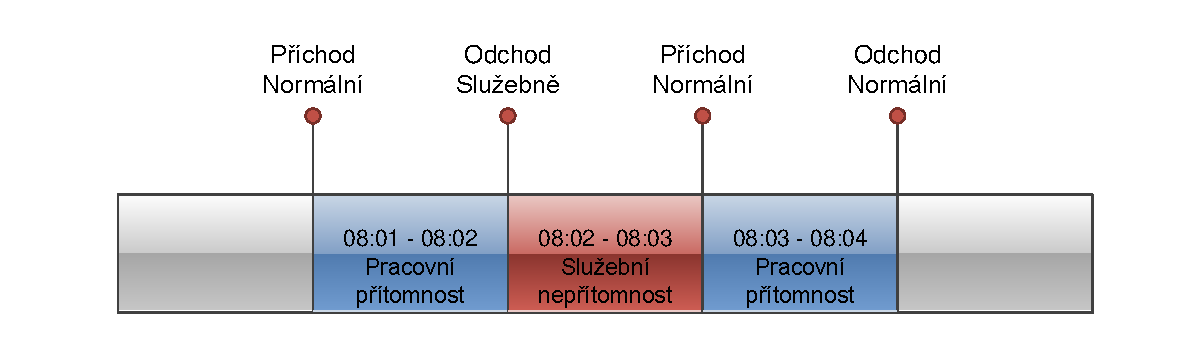
\includegraphics[scale=0.7]{visio/attservice.pdf}
\caption{Časová osa pracovního dne se služební cestou}
\label{obr:atts}
\end{figure}

\subsection{Vykazování odvedené práce}
Vykazování odvedené práce je jedním ze způsobů pro průběžnou kontrolu aktivit zaměstnanců. Ve firmě probíhá současně více projektů a bez výkazů by bylo velmi těžké sledovat průběžně náklady jednotlivých projektů. 
Díky evidenci je možné sledovat produktivitu jednotlivých zaměstnanců stejně jako nalézt slabá místa v pracovním procesu.
\\ \indent Výkazy práce jsou propojeny s docházkovým systémem a je možné porovnávat výstupy z těchto systémů. 

\subsection{Motivace}
Motivací pro vznik této práce bylo vytvořit mobilní aplikaci umožnující provádět každodenní agendu - zadávat příchody, odchody a výkazy práce pro zaměstnance, kteří často cestují a působí mimo sídlo organizace. Také snaha o využítí možností mobilního zařízení. Aplikace umožní pohodlné zadávání údajů a přinese možnost mít požadované informace po ruce.

Výsledná mobilní aplikace nemá nahradit vybrané části používaného systému, ale poskytnout efektivnější alternativu ve vybraných činnostech.

[TODO kam? pozn. původní ambice byla možnost zadávat i výkazy práce prostřednictvím mobilního klienta, vzhledem k tomu, že by bylo nutné provést úpravy v současném systému se od tohoto upustilo]

\section{Použitá technologie}
Současný systém je postaven na Oracle technologii. Jako uživatelské rozhraní používá Oracle Forms a data jsou ukládany v Oracle databázi.
 
\subsection{Oracle forms}
Oracle forms je softwarový produkt vyvinutý společností Oracle. Slouží k vytváření formulářů, které interagují s Oracle databází. Jako programovací jazyk využívá PL/SQL. Produkt byl původně používán jako terminálové rozhraní pro komuikaci se serverem. Později byl přepracován do architektury klient-server.\\ \indent
Prostředí běhu zajišťuje defaultní správu transakcí. Díky tomu je Oracle Forms silný nástroj pro efektivní vývoj aplikací, jejichž primárním cílem je přístup k datům uložených v databázi. 

\paragraph{PL/SQL}
PL/SQL (Procedural Language/Structured Query Language) je procedurální nadstavba jazyka SQL od firmy Oracle založená na programovacím jazyku Ada.

\subsection{Architektura}
Oracle Forms používá client-server architekturu. Klient funguje jako tlustý klient, který se kromě zobrazení dat stará o bussines logiku aplikace. Serverm je myšlel databázový server. Architektura je znázorněna na obr. \ref{obr:arch}

\begin{figure}[H]
  \centering
  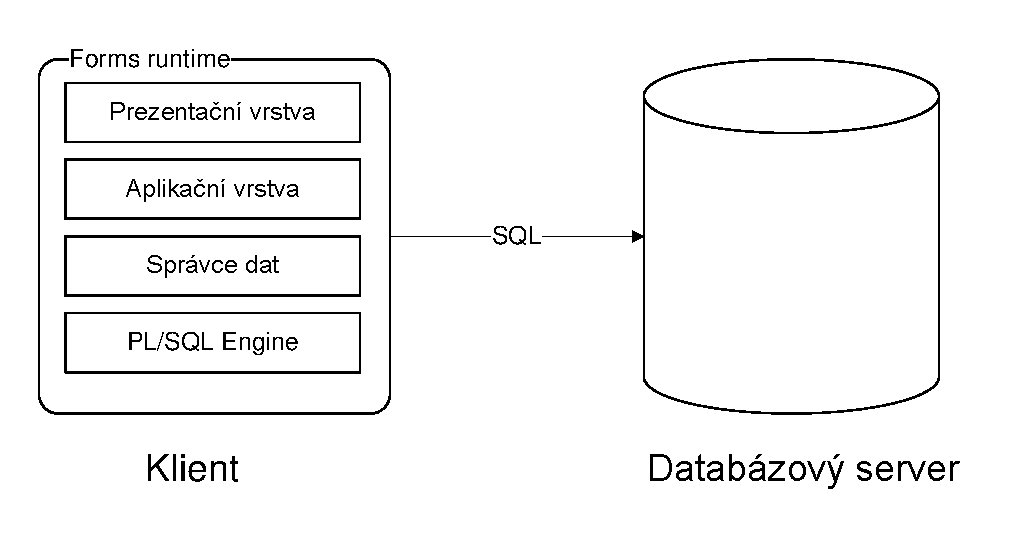
\includegraphics[scale=0.7]{visio/arch.pdf}
\label{obr:arch}
\caption{Klient-server architektura Oracle Forms aplikace}
\end{figure}
\paragraph{Forms prostředí běhu}
\begin{itemize}[noitemsep,nolistsep]
\item \textbf{Prezentační vrstva}\\
Zobrazuje informace pro uživatele formou grafického uživatelského rozhraní. Kontrolovat zadávané vstupy.
\item \textbf{Aplikační logika}\\
Stará se o provedení aplikační logiky.
\item \textbf{Správce dat}\\
Stará se o zpracování dat se kterými formulář pracuje. Řídí databázovou transakci.
\item \textbf{PL/SQL Engine}\\
Komponenta která zpracovává PL/SQL kód. Stará se o provedení procedurálního (PL) kódu a SQL kód předává ke zpracování databázi.
\end{itemize}

\paragraph{Databáze}
Databáze obsahuje data a kód, který s těmito daty pracuje (triggery, procedury, funkce). 

\subsection{Komponenty formuláře}
Z hlediska architektury se Oracle Forms aplikace skládá z těchto celků:

\subsection*{Moduly}

\paragraph{Modul formuláře} 
Modul formuláře je hlavní komponenta aplikace. Poskytuje kód nezbytný pro interakci s úložištěm a uživatelským rozhraním. 
Data poskytovaná databází jsou reflektovaná v prvcích uživatelského rozhraní jako jsou textová pole, zaškrtávací políčka, přepínače, talčítka atd. Formulář je logicky organizován do bloků. Existují dva typy bloků: 
\begin{itemize}
\item Datový blok\\ Datový blok zobrazuje zdrojová data a poskytuje abstrakci pro způsob jakým jsou tato data získávána. Blok může být asociován s databázovou tabulkou, databázovým pohledem, uloženou procedurou, dotazem do databáze nebo transakčním triggerem. Asociace datového bloku a databázových dat standartně umožnujě přístup k těmto datům a jejich modifikaci.\indent
Datové bloky mohou být navzájem svázany vztahem "rodič - potomek". Takový vztah představuje relaci 1:N databázových tabulek. Oracle Forms zajišťuje to, že při spojení mezi master a detail bloky se zobrazí pouze ty detail bloky, které jsou vázány na master blok přes cizí klíč. 

\item Řídící blok \\
Představuje blok, který nemá vztah k databázové tabulce. Řídící blok může obsahovat jakékoli prvky uživatelského rozhraní. Prvky mohou sloužit k uložení dočasných proměných nebo k zobrazení dat, které nemají přímou vazbu s databází. 
\end{itemize}

\paragraph{Modul menu} 
Modul obsahuje hiearchii menu. Každé menu obsahuje zvolitelné položky. Každý formulář obsahuje defaultní menu obsahující příkazy pro základní DML operace s databází CRUD.

\paragraph{Modul PL/SQL knihovny}
Modul obsahuje znovu využitelný kód, který může být využit jinými formuláři, menu či knihovnami. Programové jednotky knihovny mohou být fuknce, procedury a balíčky. Programové jednotky jsou spouštěny na straně klienta. Mohou obsahovat business logiku. Knihovny jsou nezávislé na formuláři, jsou zaváděny dynamicky a mohou být zároveň využívány více formuláři.

\paragraph{Modul knihovny objektů}
Modul obsahuje znovu využitelné objekty. Řeší uskladnění, správu a distribuci těchto objektů, které mohou být využity jinými formuláři, menu či knihovnami. Využívání tohoto modulu přináší přínosy v podobě úspory paměti při běhu aplikace.

\begin{figure}[H]
  \centering
  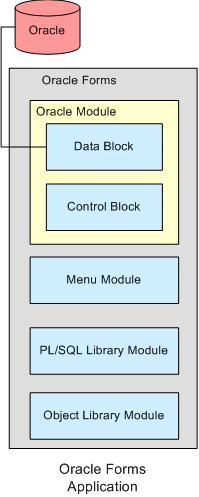
\includegraphics[scale=0.8]{obr/forms_arch3.png}
\end{figure}

\subsection*{Triggery}
Aplikace v Oracle pracuje s následujícími typy triggerů:
\begin{itemize}
\item Block-processing triggers - jsou spouštěny při události na položce patřící tomuto bloku.
\item Interface event triggers - jsou spouštěny při události v uživatelském rozhraní formuláře.
\item Master-detail triggers - jsou spouštěny při události související se vztahem "rodič - potomek"  na daných blocích. Např. při změně položky rodiče příslušný trigger zobrazí správné položky v bloku potomka.
\item Message-handling triggers - zpracovávájí zobrazení chybových či informačních zpráv.
\item Navigational triggers - jsou spouštěny při navigaci po položkách formuláře.
\item Query-time triggers - jsou spouštěny na úrovni bloku před a po dotazu do databáze.
\item Validation triggers - jsou spouštěny při validaci záznamu v položce.
\item Transactional triggers - vyvolají se při různých událostech související s interakcí s datovým úložištěm.
\end{itemize}
Pokud se jedná o datový blok, který je svázan s tabulkou v databázi, prostředí běhu automaticky zajištuje DML pro tyto bloky.
Pokud vývojář požaduje nestandartní akci při těchto úkonech, provede překrytí těchto triggerů s vlastní definovanou akcí.

\section{Uživatelské rozhraní}
\begin{figure}[H]
  \centering
  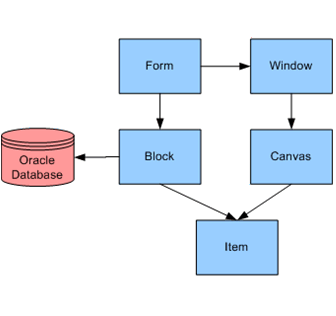
\includegraphics[scale=0.8]{obr/window.png}
\end{figure}
Plátno je objekt, na který je nakresleno celé GUI formuláře, tedy všechny viditelné objekty. Může mít prakticky jakoukoli velikost. Okno ohraničuje plochu plátna, která bude zobrazena. View řídí, jak bude plátno v určité době zobrazeno v okně.\\
TODO přepsat
\subsection*{Seznam hodnot}
Seznam hodnot je prvek uživatelského rozhraní, který uživateli nabízí výběr hodnot. Výběr může být na základě pevně daných dat či dotazem z databáze.


\newpage
\section{Důležité formuláře}

\subsection{Zápis příchodů a odchodů}
\begin{figure}[H]
  \centering
  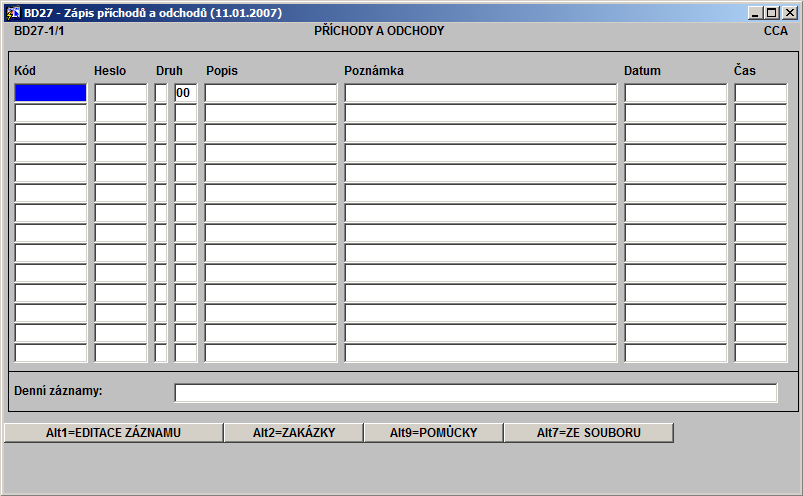
\includegraphics[scale=0.7]{obr/BD27.png}
\label{obr:att}
\caption{Formulář pro zápis příchodů a odchodů}
\end{figure}
\begin{itemize}
\item Položky bloku pro zápis docházky
\begin{description}[noitemsep,nolistsep]
\item [Kód] Identifikátor zaměstnance.
\item [Heslo] Heslo zaměstnance. Pokud heslo nemá tak prázdné pole.
\item [Druh] Druh události - příchod či odchod. Kód události.
\item [Popis] Doplní se automaticky podle kódu události.
\item [Poznámka] Volitelná poznámka.
\item [Datum] Datum události.
\item [Čas] Čas události.
\end{description}
\item Pole \emph{Denní záznamy} Zobrazuje denní docházku formou strukturovaného řetězce.
\item Pole s tlačítky Umožňuje akce které nejsou pro potřeby cílové aplikace relevantní.
\end{itemize}

\newpage
\subsection{Výkazy práce}
\begin{figure}[H]
  \centering
  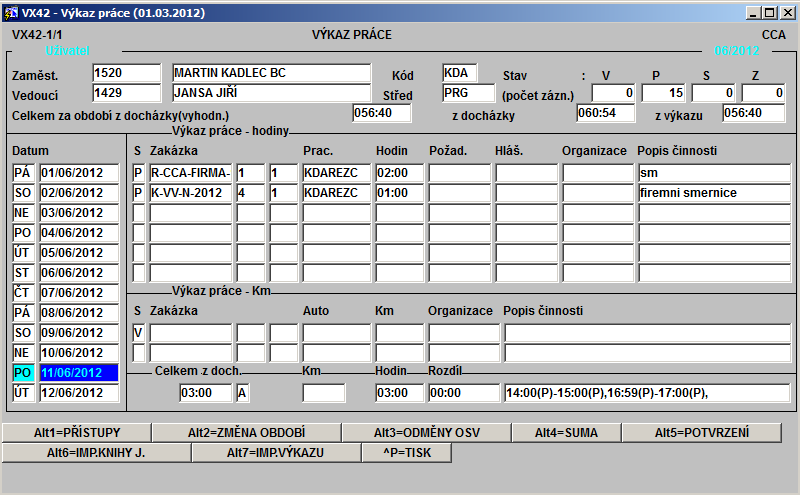
\includegraphics[scale=0.7]{obr/VX42.png}
\label{obr:rep}
\caption{Formulář pro pracovní výkazy}
\end{figure}
[TODO popsat z pohledu uzivatele]

\chapter{Analýza}

\section{Architektura}
Při návrhu architektury jsem se rozhodoval mezi třemi variantami: přímé spojení Android aplikace ke vzdálené databázi pomocí JDBC, synchronizaci dat se vzdálenou databází pomocí Oracle Database Mobile Server a nakonec využití webové služby, která by sloužila jako rozhraní mezi klientskou aplikací a databázovým serverem.

\subsection{Přímé připojení k databázi}
Přestože příme připojení k Oracle databázi pomocí JDBC je možné, tuto variantu jsem zamítl. Připojení pomocí JDBC je primárně určeno pro stabilní síťové připojení, které má malou odezvu a nízkou ztrátu paketů. Využití JDBC by přineslo problémy v podobě špatné odezvy aplikace, kvůli znovu navazování spojení a vytváření nových databázových relací, které musely být v důsledku ztráty konektivity ukončeny.\\ \indent
Vzhledem k tomu, že původní Forms aplikace funguje jako tlustý klient, provádí veškerou bussines logiku. Tato logika je zapotřebí ke správné funkčnosti systému. Bylo by tedy nutné přenést tuto logiku na stranu klienta a potřeba komunikace se vzdálenou databází by byla větší než k pouhému přenesení dat.

\subsection{Oracle Database Mobile Server}
Oracle Database Mobile Server 11g je server zajišťující  synchronizaci dat mezi Oracle databází a mobilními zařízeními. Klíčovou vlastností tohoto produktu je synchronizační jádro, které je schopné zajistit synchronizaci velké počtu mobilních zařízení se vzdálenou databázovým systémem. Přestože bylo toto synchronizační jádro navrženo pro stabilní připojení, je schopné zajistit spolehlivou funkci i při nestabilním připojení. V případě, že je spojení přerušeno synchronizace je pozastavena a po navázání spojení pokračuje v místě přerušení. Dále umožuje šifrování dat, jak pro přenos tak i pro jejich persistenci.\\ \indent
Tato varianta byla zamítnuta protože řeší pouze synchronizaci dat a neumožňuje zajistit provedení business logiky. Dalším důvodem je skutečnost, že její použití by vyžadovalo zakoupení licence pro tento server.\\ \indent
Server je možné spustit na serverech Oracle WebLogic Server a Oracle Glassfish. Mobilní klient, který běží na straně mobilního zařízení zajišťuje správu zařízení nutnou k synchronizaci. Tento klient je dostupný pro platfromy Java, Android, Blackberry, Windows a Linux.
(http://www.oracle.com/technetwork/products/database-mobile-server/overview/index.html)

\subsection{Webová služba}
Jako použitou architekturu jsem zvolil použití webové služby, která bude fungovat jako rozhraní mezi klientskou aplikací a databázovým serverem. Android klient v této architektuře funguje jako tenký klient spravující jen část funkčnosti z původního tlustého klienta. Business logika je umístěna na straně webové služby. Díky tomu že, webová služba bude umístěna v blízkosti firemní databáze, dojde k minimalizace odezev při zajištění business logiky systému. Mezi klientem a webovou službou se přenášejí pouzy data, která jsou opravdu nutná. \\ \indent
Z pohledu rozšiřitelnosti systému o další mobilní platformy se toto řešení jeví rovněž výhodně. Business logika by nebyla implementována ani na klientských aplikacích jiných platforem. Při změne logiky bude potřeba úpravy v kódu pouze na straně webové služby. Cílová architektura na vyobrazena na obrázku \ref{obr:arch}

\begin{figure}[H]
  \centering
  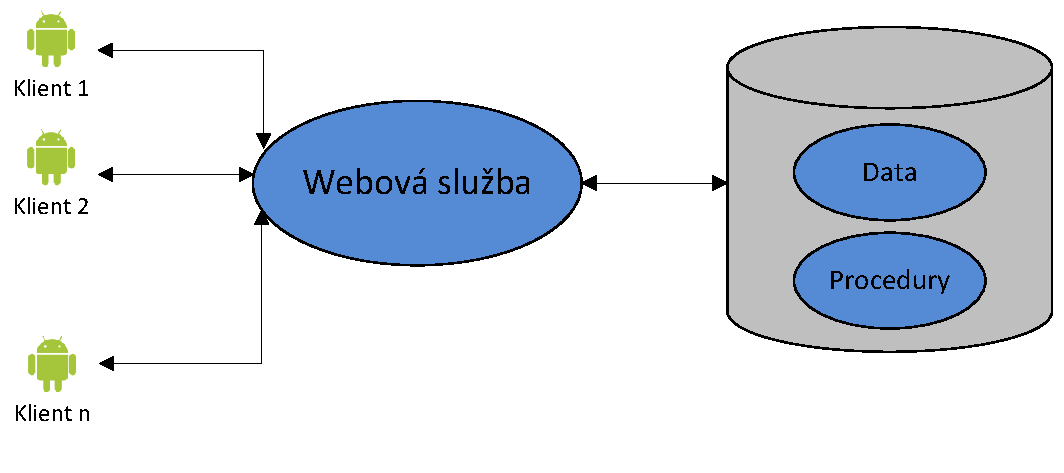
\includegraphics[scale=0.8]{obr/souc_arch2.pdf}
\caption{Zvolená architektura}
\label{obr:arch}
\end{figure}

\section{Architektura}
Android aplikace funguje jako tenký klient, který se připojuje k webové službě. Webová služba používá REST architekturu a přistupuje k samotné databázi.

\begin{itemize}
\item Webová služba - Java EE 6, aplikační server GlassFish
\item Databáze - Oracle 10g, obsahuje navíc databázové procedury, které se používají v současných formulářích  
\item Android - obsahuje persistentní úložiště, obsahuje záznamy o docházce, úložiště se bude automaticky synchronizovat ve stavu online s databázovým serverem prostřednictvím webové služby
\end{itemize}
TODO prepsat srozumitelneji
TODO schema komunikace -HHTP, JDBC

\section{Výběr typu webové služby}

\subsection{Representational State Transfer}

\subsection{Simple Object Access Protocol}

\section{Datová vrstva}
V této kapitole analyzuji datovou vrstvu systému. 

\subsection{Datový model}
V následujícím diagramu (obr. \ref{obr:object}) zobrazuji entity nacházející se v systému, které jsou relevantní pro zkoumanou část systému. Další tabulky a číselníky jsou pro jednoduchost vypuštěny.
\begin{figure}[H]
  \centering
  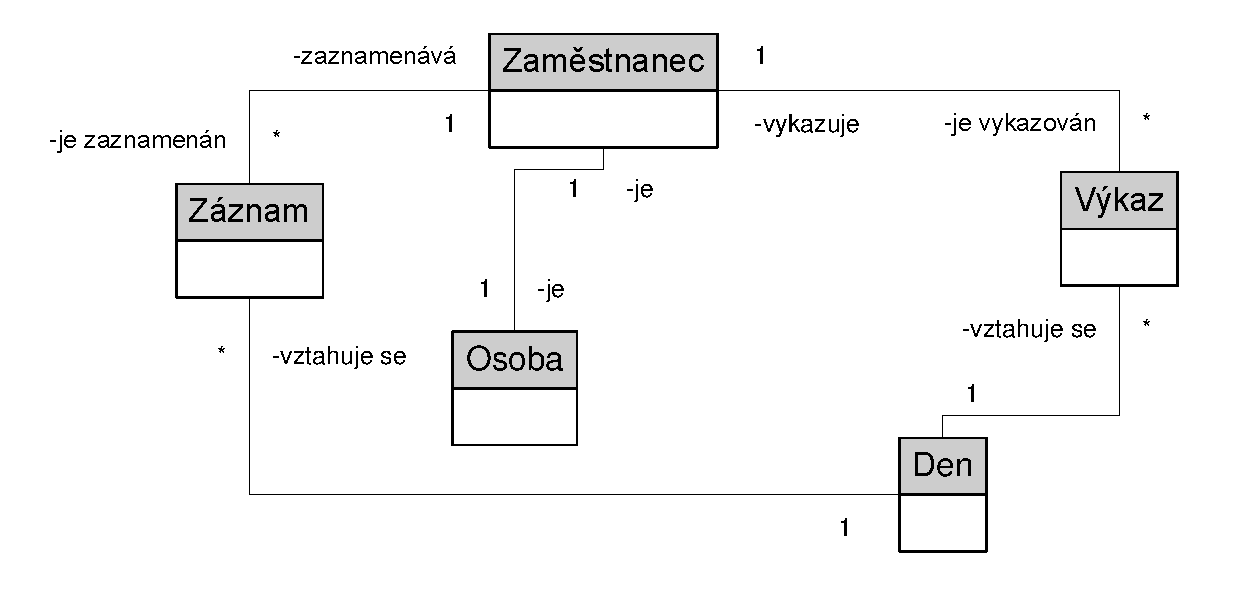
\includegraphics[scale=0.7]{visio/object.pdf}
\caption{Diagram relevantních entit nacházejících se v systému}
\label{obr:object}
\end{figure}
Jednotlivé entity a jejich popis:
\begin{itemize}
\item Záznam\\
Příchod nebo odchod na pracoviště. Obsahuje informaci o čase, datu, účelu a případně zaměstnancův krátky popis události.
\item Výkaz\\
Pracovní výkaz. Obsahuje informaci o čase, datu, osobě zadavatele, osobě řešitele, vykazované době, vazbu na zakázku či chybové hlášení, stav výkazu, zaměsnancův popis činnosti.
\item Zaměstnanec\\
Zaměstnanec a jeho příslušnost k pracovnímu oddělení, funkce, vedoucí pracovník a typ úvazku. 
\item Osoba\\
Podrobnější informace o osobě zaměstnance, jméno, pracovní zkratka.
\item Den\\
Rozlišení pracovních dnů a svátků.
\end{itemize}

\subsection{Práce s datumem a časem}
Při návrhu datového modelu jsem řešil problém pomocí jakého datového typu vyjadřovat údaj o čase či datu. V Oracle databázi je použit datový typ Date. SQLite databáze nabízí tři způsoby jako ukládat informaci o čase:
\begin{itemize}
\item \textbf{TEXT} podle ISO8601 normy ve formátu "YYYY-MM-DD HH:MM:SS.SSS".
\item \textbf{REAL} podle Juliánského kalendáře, počet dní od poledne 24. Listopadu roku 4714 před kristem (Greenwichského času).
\item \textbf{INTEGER} jako Unix Time, počet sekund 1970-01-01 00:00:00 UTC.
\end{itemize}

\noindent
Pro uložení v SQLite databázi jsem zvolil typ INTEGER. V aplikaci (Android klient, webová služba) jsem se rozhodl reprezentovat časový údaj pomocí primitivního typu long. Měl jsem k tomu řadu dobrých důvodů:
\begin{itemize}
\item odpadá starost s formátem datumu při serializaci a deserializace JSON řetězce
\item snadné porovnávání hodnot pomocí relačních operátorů
\item sníží se počet konverzí v aplikaci (např. pro výpočet pozice pro vykreslení komponenty v UI)
\end{itemize}

Také jsem se ujistil, že rozsah typu long je pro potřeby aplikace dostačující. Srovnání použitých datových typů je znázorněno v tabulce \ref{tab:cas}. 

\begin{table}[H]
\centering
\begin{tabular}{| c | c | c | c |}
\hline
Datový typ &  Minimální hodnota & Maximální hodnota & Přesnost \\ \hline
Oracle Date &   January 1, 4712 BCE  &  December 31, 4712 CE &  sekundy \\ \hline
SQLite INTEGER &    &  &  sekundy \\ \hline
Java long & 2.12.292269055 BC   & 17.8.292278994 AD &  milisekundy \\ \hline
\end{tabular}
\caption{Datové typy reprezentující časový údaj}
\label{tab:cas}
\end{table}

\subsection{Kritika datové vrstvy}
co se mi nelibilo a co bych navrhl jinak a jak, navrh prichody/odchody - jeden radek,
chybi primarni klic - ROWID jako unikatni identifikator, problemy ktere to prinasi,
format casu - problemy s prevodem

\section{Business logika}
existuje někajá možnost převodu formsů do javy - oracle adf - co to je, co to resi, proc to neresi muj problem\\
prijde to do webove sluzby - duvody
\subsection{Triggery}
jen ty, jejichž funkčnost bude muset být implementována.
\begin{itemize}
\item On-Delete, On-Insert, On-Update, Pre-Delete, Pre-Insert, Pre-Update
\item When-Validate-Item
\end{itemize}

\subsection{Databázové balíčky a uložené procedury}
ukázky volání z javy
\subsection{Forms knihovny}

\section{Synchronizace dat}
V současném systému uživatel zadává data prostřednictvím příslušného formuláře. Změny jsou aplikovány bezprostředně po uložení během databázové transakce. Mobilní klient přináší nový způsob použití - data lze zadat i v režimu offline, kdy mobilní klient není v dosahu webové služby. Tyto data jsou uložena persistentně na straně klienta a jsou synchronizována až ve chvíli kdy je možná komunikace s webovou službou.\\ \indent
Synchronizace se týká pouze dat pro docházku uživatele. Ostatní data jsou prostřednictvím mobilního klienta pouze zobrazována. Je třeba počítat s tím, že záznamy přidané na straně klienta v režimu offline nemusí být přijaty při synchronizaci z důvodu porušení business pravidel a uživatel by měl být o této skutečnosti vhodně informován.

\subsection{Obousměrná synchronizace}
Při obousměrné synchronizaci se odesílají data ze strany klienta na server tak i opačným směrem ze serveru na klienta. Klienta lze navrhnout tak, aby si uchovával informaci o změnách na svojí straně. Při analýze databázového schématu pro docházku v současném systému jsem zjistil, že databáze neuchovává informaci o změnách na svojí straně. Beze změny této skutečnosti není možné sledovat změny na straně databáze. Výsledkem je poněkud neefektivní způsob synchronizace, kdy klient odesílá na server pouze změny, zatímco ze serveru stahuje všechna data pro daného uživatele a období.
\\ \indent
Celkový průběh synchronizace je znázorněn v diagramu \ref{obr:sync}. Klient nejprve odešle všechny svoje změny na server. Poté smaže všechny úspěšně odeslaná data. Bez smazání by nebylo možné zjistit, že na serveru došlo ke změně či smazání dat jiným klientem. Poté už zbývá pouze stažení aktuálních dat ze serveru. Data která na klientovi nebyla smazána z důvodu neúspěsného odeslání na server, zůstávají do té doby, než uživatel tyto data upraví tak aby vyhovovali bussines pravidlům. Dalším důvodem pro neúspěšnou synchronizaci může být přerušení spojení. Data zůstavají na klientovi, až do doby úspěšného pokusu o synchronizaci.
\begin{figure}[H]
  \centering
  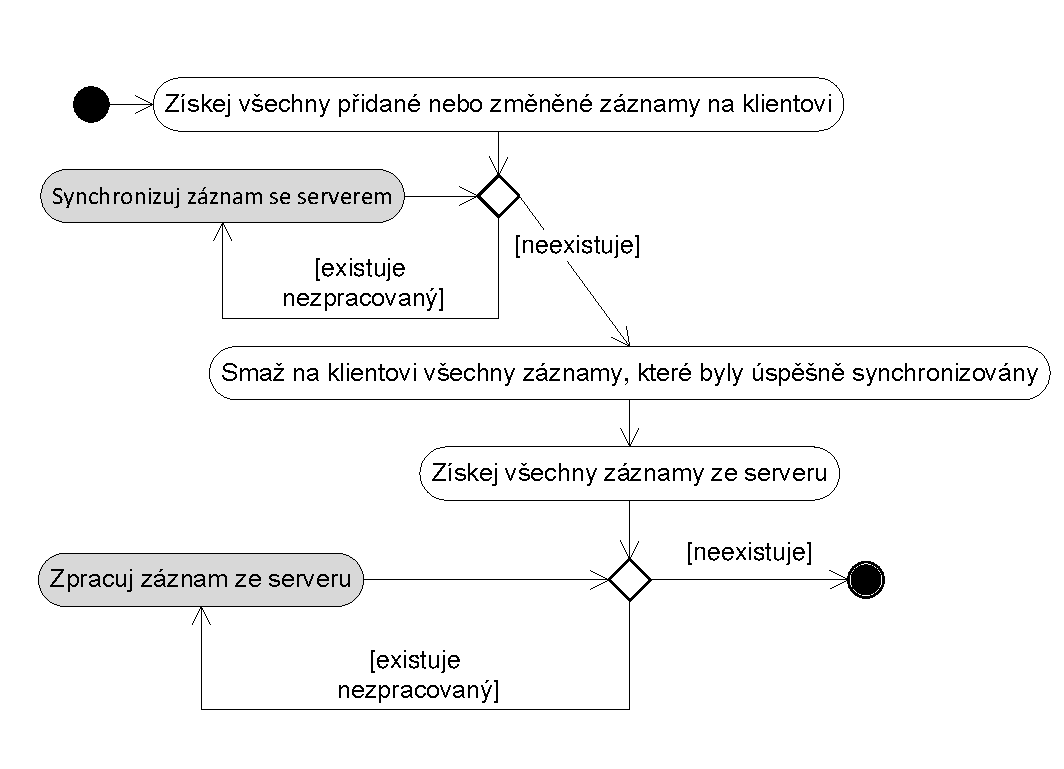
\includegraphics[scale=0.7]{visio/sync.pdf}
\caption{Diagram aktivit pro průběh synchronizace}
\label{obr:sync}
\end{figure}

Diagram \ref{obr:syncup} podrobněji rozepisuje průběh odeslání požadavku na server. Pokud klient nemá server ID záznamu, znamená to, že záznam byl vytvořen na straně klienta a odesílá se požadavek na vytvoření. Pokud klient zná server ID může požadovat smazání nebo aktualizaci záznamu. 

\begin{figure}[H]
  \centering
  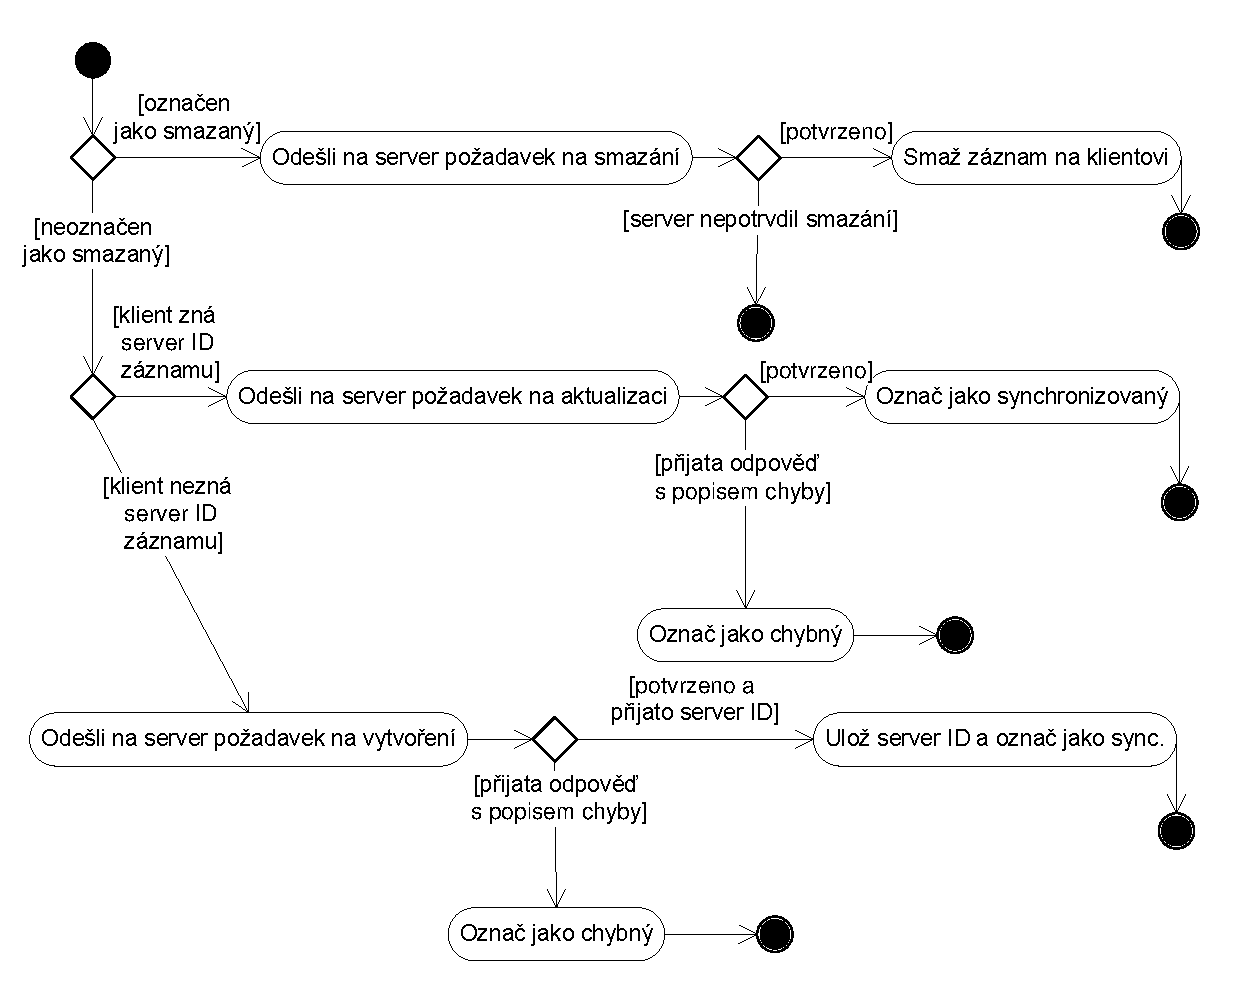
\includegraphics[scale=0.7]{visio/syncup.pdf}
\caption{Diagram aktivit pro odeslání požadavku na server}
\label{obr:syncup}
\end{figure}

Diagram \ref{obr:syncup} podrobněji rozepisuje průběh přijetí záznamu ze serveru.
TODO popsat kolizi
\begin{figure}[H]
  \centering
  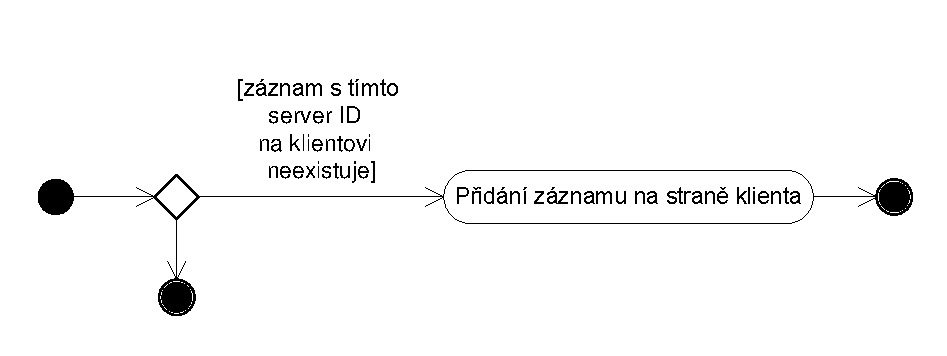
\includegraphics[scale=0.7]{visio/syncdown.pdf}
\caption{Diagram aktivit pro přijetí záznamu ze serveru}
\label{obr:syncdown}
\end{figure}

\subsection{Obousměrná synchronizace s úpravou databáze}
Jiná varianta řešení problému synchronizace dat, která se snaží eliminovat nedostatky předchozí varianty, by vyžadovala změny v databázovém schématu současného systému. U každého záznamu by byla přidána informace o poslední změně záznamu s vhodnou časovou přesností. Pokud by došlo k požadavku na smazání záznamu, nebyl by záznam skutečně smazán, ale pouze nastaven přížnak smazaného záznamu. Při použití tohoto řešení by bylo možné synchronizovat oběma směry pouze změny ze strany klienta i serveru. \\ \indent
Klient který iniciuje synchronizaci nejprve odešle na server požadavek ke kterému připojí údaj o času provedení poslední synchronizace. Server odesílá ke klientovi pouze ty data, která se změnila po tomto termínu. Poté klient odesílá svoje změny na server.

\subsection{Řešení kolizí}
Kolize teoreticky nastane vždy, když se v době od poslední synchronizace změní stejná data jak na serveru, tak v zařízení. Vzhledem k tomu, že server neukládá informaci o čase poslední synchronizace a není tedy možné zjistit že vůbec došlo ke změne dat, tak mobilní klient vždy přepíše záznam na serveru.

\subsection{Srovnání}
V obou případech řešení je iniciátorem synchronizace klient. Druhá varianta by oproti první přinesla úsporu množství přenesených dat. Vzhledem k tomu, že druhá varianta by vyžadovala změnu v databázovém schématu současného systému, zvolil jsem první variantu i přesto, že z hlediska efektivity synchronizace je to horší řešení.

\section{Uživatelské rozhraní}
zarizeni zna identitu uzivatele, nezadava zbytecnosti

\chapter{Zabezpečení}
V následující kapitole se zabývám zabezpečením aplikace. Popisuji několik možných variant z hlediska ověřování identity uživatele. Na závěr vysvětluji výběr zvoleného řešení.
\section{Autentizace a autorizace}
Při analýze současného systému jsem zjistil, že informace o docházce a výkazech zaměstnanců jsou dostupné všem ostatním uživatelům (údaje týkající se nadřízených pracovníků jsou dostupné i podřízením). Dalším zajímavostí je, že heslo používané k zadání docházky je pro uživatele nepovinné (má ho jen ten uživatel, který si ho nastavil). 

\subsection*{Autentizace}
Autentizace je proces ověření proklamované identity subjektu. Uživatel se identifikuje pomocí svého uživatelského jména a hesla.

\subsection*{Autorizace}
Autorizace je proces získávání souhlasu s provedením nějaké operace. Uživatel musí zadávat svoj přístupové údaje při zadání každého záznamu docházky. 

\subsection*{Riziko poškození systému}
Webová služba umožňuje čtení a úpravu docházkových dat a dále čtení dat o výkazech práce a zaměstnancích. Dále používá některé databázové objekty jako jsou procedury a funkce, které pracují s těmito daty. Je vhodné aby aplikace měla přístup pouze k těm databázovým objektům, které jsou relevantní pro navrženou funkčnost aplikace. To je vhodné pro maximální zabezpečení okolního systému a minimalizaci případných rizik při zneužití či chybě v aplikaci. Toto je zodpovědností databázového administrátora organizace a v této práci se touto problematikou dále nezabývám.

\subsection*{HTTP Basic autentizace}
Klient posílá autentizační hlavičku jako součást HTTP požadavku na server. Jméno a heslo je zasláno jako jeden textový řetězec oddělený dvojtečkou. Výsledný řetězec je poté zakódován metodou Base64. Uživatelské jméno a heslo se tedy posílá v zakódované podobě. Nejedná se ale o kryptografické zabezpečení přihlašovacích údajů. Použití této metody předpokládá použití zabezpečeného komunikačního kanálu mezi klientem a serverem.


\section{VPN pro vzdálený přístup}
Virtuální privátní síť  je prostředek pro propojení počítačů v prostředí nedůvěryhodné sítě. Díky VPN spojení mohou počítače komunikovat tak, jako by byly součástí důvěryhodné sítě.

\subsection*{Vlastnosti připojení VPN}
\begin{itemize}[noitemsep,nolistsep]
\item Zapouzdření\\ Při použití technologie VPN jsou data zapouzdřena pomocí hlavičky obsahující směrovací informace, které umožňují průchod dat přes tranzitní síť.
\item Ověřování\\
Klient a VPN server se vzájemně ověřují na úrovni počítače. Android má integrovanou podporu pro VPN využívající protokoly PPTP, L2TP a IPSec.
\item Šifrování dat\\
Pro utajení dat během jejich přenosu sdílenou nebo veřejnou tranzitní sítí jsou data na straně odesílatele zašifrována a na straně příjemce dešifrována. Šifrování a dešifrování je založeno na tom, že odesílatel i příjemce používají společný šifrovací klíč.
\end{itemize}

Webová služba je tedy umístěna na serveru uvnitř firemní sítě. Pokud klient chce komunikovat s webovou službou musí tak činit 
prostřednictvím sítě VPN.

\section{Autentizace proti databázi}
Klient i server jsou součástí jedné VPN sítě, která zajišťuje důvěryhodný komunikační kanál.  Klient posílá na server HTTP požadavek jehož součástí je autentizační hlavička nesoucí uživatelské jméno a heslo. Webová služba ověří jméno a heslo pomocí databázové procedury. Jméno a heslo uživatele je uloženo v databázi. Implementované řešení je znázorněno na obr. \ref{obr:auth} který zobrazuje sekveční UML diagram v případě úspěšné autentizace.
\begin{figure}[H]
  \centering
  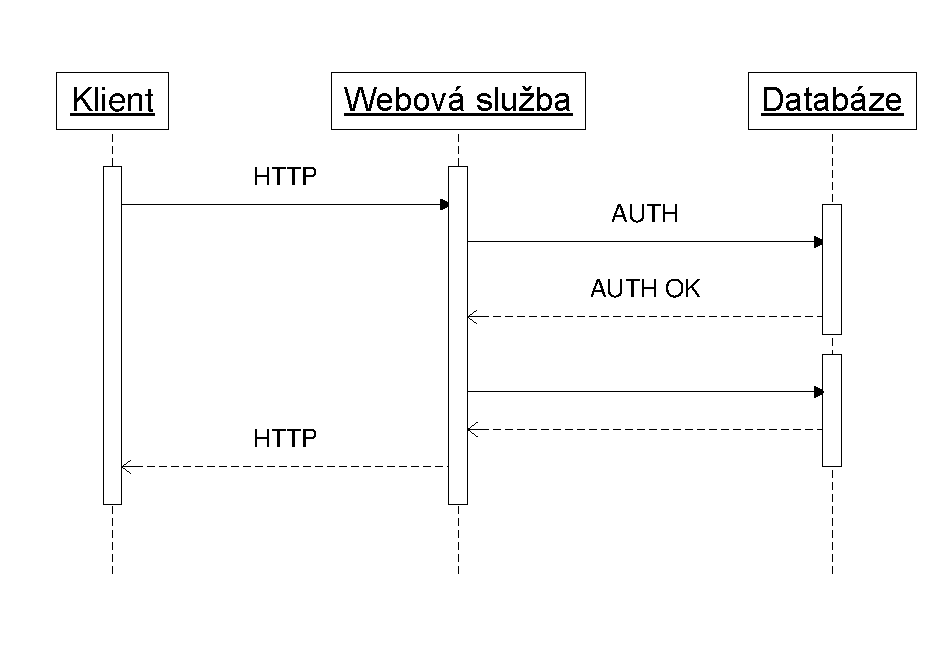
\includegraphics[scale=0.8]{visio/auth.pdf}
\caption{Diagram aktivit při úspěšné autentizaci}
\label{obr:auth}
\end{figure}

\section{Autentizace proti LDAP}
Alternativním řešením by bylo ověřování uživatelů pomocí LDAP adresáře. Organizace již LDAP používá v některých dalších firemních systémech. Toto řešení se liší v tom, že dotaz na ověření identity uživatele probíhá k LDAP adresáři a nikoli k databázi. Implementované řešení je znázorněno na obr. \ref{obr:authldap}, který zobrazuje sekveční UML diagram v případě úspěšné autentizace.
\begin{figure}[H]
  \centering
  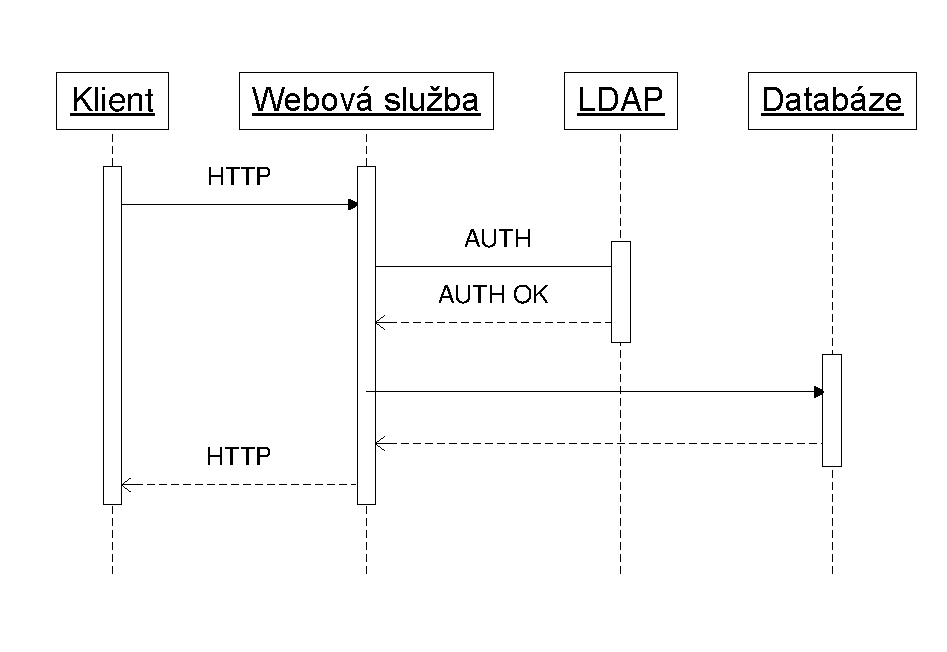
\includegraphics[scale=0.8]{visio/auth_ldap.pdf}
\caption{Diagram aktivit při úspěšné autentizaci}
\label{obr:authldap}
\end{figure}
\subsection{LDAP}
 Directory Access Protocol (LDAP) je internetový protokol definující přístup k distribuované adresářové službě. Podle tohoto protokolu jsou jednotlivé položky na serveru ukládány formou záznamů a uspořádány do stromové struktury. Protokol LDAP je byl navržen v souladu  se sadou standartů X.500 vyvinutých pro adresářové služby v počítačových sítích. Protokol LDAP je jejich odlehčenou verzí.\\ \indent
Aplikace funguje na bázi klient-server. Klient se při komunikaci se serverem autentizuje. Prostřednictvím klienta lze přidávat, modifikovat a mazat záznamy na serveru.

\subsection*{Schéma}
Úkolem informačního modelu LDAP je definovat datové typy a informace, které lze v adresářovém serveru ukládat. Data jsou uchovávána ve stromové struktuře pomocí záznamů. Záznam představuje souhrn atributů (dvojice jméno - hodnota). Atributy nesou informaci o stavu daného záznamu. Záznamy, uložené v adresáři, musí odpovídat přípustnému schématu. Schéma  představuje soubor povolených objektových tříd a k nim náležících atributů.\\
Ukázka schématu definující strukturu záznamu zaměstnance:
\begin{verbatim}
objectclass ( 1.1.2.2.2 NAME 'zamestnanec'
                DESC 'zamestnanec firmy'
                SUP osoba
                MUST ( jmeno $ identifikacniCislo )
                MAY zkratkaZamestnance )
\end{verbatim}

Objekt popisující zaměstnance dědí od objektu osoba, vyžaduje povinný atribut 'jmeno' a 'identifikacniCislo' a nepovinný atribut 'zkratkaZamestnance'.

\subsection*{Funkční model}
Funkční model umožňuje pomocí základních operací manipulovat a přistupovat k záznamům v adresáři a měnit či zjišťovat tak jejich stav.
\begin{itemize}[noitemsep,nolistsep]
\item Autentizační operace: Slouží k přihlášení a odhlášení uživatele pro komunikaci s adresářovým serverem. Jsou jimi míněny především operace bind a unbind. Na úspěšném provedení operace bind závisí výsledky aktualizačních a dotazovacích operací nad adresářem.
\item Aktualizační a dotazovací operace: Každý adresářový server podporuje základní operace s daty, jako je vyhledávání, přidávání, mazání, porovnávání a modifikace záznamů. Tyto operace bývají často spjaté s nastavením bezpečnostního modelu.
\end{itemize}

\subsection*{LDAP URL}
Umístění zdroje je v LDAP specifikováno pomocí URL, které má následující tvar:
\begin{verbatim}
ldap://host:port/DN?attributes?scope?filter?extensions
\end{verbatim}
\begin{itemize}[noitemsep,nolistsep]
\item host - doména nebo IP adresa
\item port - síťový port (defaultně 389)
\item DN - význačné jméno použité jako základ pro vyhedávání
\item attributes -  seznam atributů
\item scope - specifikuje vyhledávácí rozsah  
\item filter - filtrovací kritérium
\item extensions - rozšíření
\end{itemize}

\section{Shrnutí}
Hlavním prvkem zabezpečení je VPN přístup. Uživatel bez přístupu do firemní VPN nemůže komunikovat s webovou službou. Od uživatele se očekává, že si nakonfiguruje VPN připojení v nastavení Android mobilního zařízení.\\ \indent
Použil jsem první řešení protože je shoduje se způsobem ověřování v současném systému. Stávají řešení pomocí Oracle Forms aplikace používá rovněž ověření uživatele dotazem k databázi tzn. ověření se děje na aplikační vrstvě. \\ \indent
Je nutné dívat se na pravidlo dobrovolného hesla jako na firemní pravidlo, které může být kdykoli zrušeno. V případě zrušení tohoto pravidla by se z největší pravděpodobností uplatnilo ověřování proti LDAP adresáři. 

\chapter{Webová služba}

\section{REST}
Při návrhu REST služby jsem nejprve identifikoval všechny zdroje, které webová služba zpřístupňuje. Jedná se o údaje o docházce zaměstnanců, výkazech práce a zaměstnancích samotných. Posledním zdrojem je možnost testovat komunikaci s webovou službou. \par
Zdroj pro docházku zaměstnaců tzn. jejich příchody a odchody (označované jako události) a poskytované služby zobrazuje tabulka \ref{tab:urievents}. Služba umožňuje operace CRUD na datovém zdroji zaměstnanců a dále zjištění součtu doby v zaměstnání.

\definecolor{Gray}{gray}{0.9}
\renewcommand{\arraystretch}{1.5}
\begin{table}[H]
\begin{center}
\begin{tabular}{| m{2cm} |  m{10cm} |}
\hline
\rowcolor{Gray}
GET & events/\{icp\}?from=\{from\}\&to=\{to\} \\ \hline
&  \parbox{10cm}{Získá všechny události zaměstnance za dané období\\
Parametry:\begin{itemize}[noitemsep,nolistsep]
\item icp - identifikátor zaměstnance
\item from - datum začátku období
\item to - datum konce období
\end{itemize}} \\ \hline
\rowcolor{Gray}
DELETE  & events/\{rowid\} \\  \hline
&  \parbox{10cm}{Smaže danou událost\\
Parametry:\begin{itemize}[noitemsep,nolistsep]
\item rowid - identifikátor události
\end{itemize}} \\ \hline
\rowcolor{Gray}
POST  & events \\  \hline
&  \parbox{10cm}{Vytvoří událost, používá se bez parametrů protože identifikátor pro událost vytváří server
} \\ \hline
\rowcolor{Gray}
PUT  & events/\{rowid\} \\ 
&  \parbox{10cm}{Aktualizuje danou událost\\
Parametry:\begin{itemize}[noitemsep,nolistsep]
\item rowid - identifikátor události
\end{itemize}} \\ \hline
\rowcolor{Gray}
GET & events/sum/\{icp\}?from=\{from\}\&to=\{to\} \\ \hline
&  \parbox{10cm}{Získá součet přítomnosti zaměstnance za dané období\\
Parametry:\begin{itemize}[noitemsep,nolistsep]
\item icp - identifikátor zaměstnance
\item from - datum začátku období
\item to - datum konce období
\end{itemize}} \\ \hline
\end{tabular}
\end{center}
\caption{Služby pro události docházky}
\label{tab:urievents}
\end {table}

\noindent
Zdroj pro údaje o zaměstnancích
\begin{table}[H]
\begin{center}
\begin{tabular}{| m{2cm} |  m{10cm} |}
\hline
\rowcolor{Gray}
GET  & employees/\{icp\} \\ \hline
&  \parbox{10cm}{Získá údaje o zaměstnaci identifikovém pomocí parametru\\
Parametry:\begin{itemize}[noitemsep,nolistsep]
\item icp - identifikátor zaměstnance
\end{itemize}} \\ \hline
\hline
\rowcolor{Gray}
GET  & employees/all/\{icp\} \\ \hline
&  \parbox{10cm}{Získá seznam všech zaměstnanců, kteří jsou aktuálně v zaměstnaneckém poměru, obsahuje informaci zda jsou tito zaměstnanci podřízení, vzhledem k zaměstnanci identifikovém pomocí parametru\\
Parametry:\begin{itemize}[noitemsep,nolistsep]
\item icp - identifikátor zaměstnance
\end{itemize}} \\ \hline
\rowcolor{Gray}
GET  & employees/lastevents \\ 
&  \parbox{10cm}{Získá poslední událost v docházce všech zaměstnanců, kteří jsou aktuálně v zaměstnaneckém poměru}\\
\hline
\rowcolor{Gray}
GET  & employees/lastevents/\{icp\} \\ 
&  \parbox{10cm}{Získá poslední událost v docházce zaměstnance identifikovém pomocí parametru}\\
\hline
\end{tabular}
\end{center}
\caption{Služby pro zaměstnance}
\label{tab:uriemps}
\end{table}
\noindent

Zdroj výkazy práce
\begin{table}[H]
\begin{center}
\begin{tabular}{| m{2cm} |  m{10cm} |}
\hline
\rowcolor{Gray}
GET  &records/\{kodpra\}?from=\{from\}\&to=\{to\} \\ 
&  \parbox{10cm}{Získá všechny výkazy práce zaměstnance za dané období\\
Parametry:\begin{itemize}[noitemsep,nolistsep]
\item kodpra - identifikátor zaměstnance (zkratka)
\item from - datum začátku období
\item to - datum konce období
\end{itemize}} \\ \hline
\rowcolor{Gray}
GET & records/sum/\{icp\}?from=\{from\}\&to=\{to\} \\ \hline
&  \parbox{10cm}{Získá součet vykázaného času zaměstnance za dané období\\
Parametry:\begin{itemize}[noitemsep,nolistsep]
\item icp - identifikátor zaměstnance
\item from - datum začátku období
\item to - datum konce období
\end{itemize}} \\ \hline
\end{tabular}
\end{center}
\caption{Služby pro výkazy práce}
\label{tab:urirecords}
\end{table}

\section{Filtry}

\section{web.xml}

\chapter{Android aplikace}

\section{Funkcionalita}
[TODO ještě upřesnit]
Na základě analýzy současného systému a potřeb zaměstnanců byla vybrána k implementaci následující funkčnost: 
\paragraph{Docházka}
\begin{itemize}
\item Přehledné zobrazení událostí docházky daného zaměstnance
\item Uživatel má možnost přidávat, ediovat a mazat svoje události
\item Aplikace zajišťuje automatickou synchronzaci těchto údajů s firemní databází
\item Zobrazení poměru typů docházkových událostí za dané období
\end{itemize}
\paragraph{Aktuální přítomnost na pracovišti}
\begin{itemize}
\item Zobrazení seznamu zaměstnanců aktuálně přítomných na pracovišti
\item Uživatel má možnost spravovat seznam svých "oblíbených" zaměstnanců a tento seznam zobrazovat přednostně
\end{itemize}
\paragraph{Výkazy práce}
\begin{itemize}
\item Zobrazení poměru typů zakázek za dané období
\item Zobrazení vývoje vývoje daného typu zakázky v daném období 
\item Možnost zobrazení těchto údajů i za jiné zaměstnance
\end{itemize}

\subsection{Nastavení a konfigurovatelnost}
Aplikace si musí pamatovat údaje nutné pro snadnou obsluhu tzn. uživatelské jméno a heslo, adresu umístění webové služby a tyto údaje jsou konfigurovatelné.\\
Dále aplikace umožní uživateli konfigurovat vzhled některých kompoment, jako je barva typu události v docházce a typu záznamu ve výkazech.

\subsection{Uživatelská přívětivost}
Uživatelské rozhraní aplikace klade důraz na přehlednost, ergonomii a časově efektivní obsluhu.

\subsection{Návrhy na vylepšení}

\section{Komponenty Android aplikace}

\subsection{Aktivita}
Aktivita představuje jednu obrazovku s uživatelským rozhraním. Každá akvitita umožňuje nějakou funkčnost. Příkladem aktivit použitých v implementované aplikaci může být zobrazení denní docházky uživatele, kalendář umožňující výběr data, přidání a editace docházkové události nebo uživatelské nastavení.

\subsubsection*{Životní cyklus aktivity}
Aktivita se může nacházet ve třech stavech:

\begin{itemize}[]
\item \textbf{Běžící}\\
Aktivita je na popředí a umožňuje interakci s uživatelem.
\item \textbf{Pozastavený}\\
Na popředí se dostala jiná aktivita. Pozastavená aktivita je stále viditelná, ale je překrytá novou aktivitou. Pozastavená aktivita nemůže provádět interakci s uživatelem. Objekt aktivity zůstává v paměti, je zachována veškerá stavová informace. Při nedostatku systémové paměti může být aktivita zničena.
\item \textbf{Zastavený}\\
Aktivita není viditelná. Objekt aktivity zůstává v paměti, je zachována veškerá stavová informace. Při nedostatku systémové paměti může být aktivita zničena.
\end{itemize}

\subsubsection*{Metody životního cyklu aktivity}
Při přechodech aktivity mezi výše uvedenými stavy dochází k volání callback metod. Tyto metody jsou volány systémem. Každá  
z metod má defaultní chování. Programátor může libovolnou z metod překrýt v případě, že požaduje jinou funkcionalitu, ale musí mít na paměti, že většina z nich vyžaduje volání metody rodiče.
\begin{itemize}[]
\item \textbf{onCreate()}\\
Metoda je volána v okamžiku, kdy je aktivita poprvé vytvořena. Zde se připraví prvky uživatelského rozhraní a nastaví se zdroje dat. Pokud existuje uložený stav aktivity z dřívější doby, může být využit. 
\item \textbf{onRestart()}\\
Volána pokud se aktivita před tím nacházela ve stavu \emph{Zastavený} a má se dostat do stavu \emph{Běžící}.
\item \textbf{onStart()}\\
Volána před tím, než se aktivita stane viditelnou.
\item \textbf{onResume()}\\
Volána před tím, než je uživatelovi umožněna interakce s aktivitou. Aktivita se dostává na vrchol zásobníku aktivit aplikace.
\item \textbf{onPause()}\\
Volána ve chvíli kdy se má jiná aktivita dostat na popředí. V této metodě by měla být uložena veškerá rozpracovaná data a ukončeny úkoly, které si zabírají výpočetní výkon. Nová aktivita není spuštěna, dokud tato metoda není dokončena.
\item \textbf{onStop()}\\
Po volání metody není aktivita nadále viditelná. K volání dochází v situaci, kdy je aktivita ukončována nebo se jiná aktivita dostala do popředí.
\item \textbf{onDestroy()}\\
Volání před tím než je aktivita ukončena. K volání dochází v případě, že aktivita končí svoji činnost nebo v situaci, kdy se systém dožaduje systémových prostředků.
\end{itemize}

\subsubsection*{Ukládání stavu aktivity}
Ukládat stav aktivity je vhodné protože systém může zničit aktivitu z důvodu nedostatku paměti. Další důvodem je situace, kdy uživatel změní orientaci obrazovky. V takové situaci nezůstává v paměti objekt aktivity, ale aktivita musí být znovu vytvořena. Uživatel samozřejmě očekává, že aktivitu nalezne ve stejném stavu v jakém ji opustil. K těmto účelům jsou určeny dvě callback metody:

\begin{itemize}[]
\item \textbf{onSaveInstanceState(Bundle)}\\
Metoda je volána před tím než je aktivita zničena (před provedením \emph{onStop()}. Do objektu \emph{Bundle} by měla být uložena všechna data, která jsou nutná pro obnovu předchozího stavu aktivity. Data jsou ukládána ve formátu klíč-hodnota. Metoda není volána v situaci kdy uživatel explicitně ukončil aktivitu. Na začátku metody je nutné zavolat metodu rodiče, aby mohl být uložen stav prvků UI pomocí defaultní implementace.
\item \textbf{onRestoreInstanceState(Bundle)}\\
Metoda je volána (po provedením \emph{onStart()} v případě, že aktivita byla znovuobnovena z předchozího uloženého stavu.Na začátku metody je nutné zavolat metodu rodiče, aby mohl být obnoven stav prvků UI pomocí defaultní implementace.
\end{itemize}


\subsection{Fragment}
\subsection{Služba}
+ restart zařízení?
\subsection{Content provider}
\subsection{Broadcast receiver}

\begin{enumerate}
\item komponenty pro sync a auth, provazani s android ucetm
\item CursorLoader
\item Async task
\item  nestandartni UI
\item modifilkace adapterview
\item cutom UI - viewgroup
\item widgety
\item alarmanager
\item handler - hlavni vlakno
\item activity - dedicnost
\end{enumerate}
+ nejaka ukazka konkretniho pouziti

\section{Komponenty pro synchronizaci}
\begin{enumerate}
\item sync architektura - komponenty
\end{enumerate}



\section{Uživatelský účet}
Android poskytuje správu účtů pro online služby. Uživatel zadá svoje přihlašovací údaje při vytvoření účtu a dává tak aplikaci svolení k využívání tohoto účtu.\\ \indent
Různé online služby mohou využívat odlišný způsob pro autentizaci. Android manažer účtů využívá kompomentu \emph{authenticator} \cite{accman}, která je obvykle poskytována třetí stranou - poskytovatelem dané služby. Příkladem služby, která poskytuje vlastní \emph{authenticator} je např. Google, Facebook a Microsoft Exchange.\\ \indent
Nejdůležitější třída pro práci s účty je \emph{AccountManager}. Zde je výčet nejdůležitějších metod:
\begin{itemize}[]
\item \textbf{addAccountExplicitly(Account account, String password, Bundle userdata)}\\
Vytvoří nový účet.
\item \textbf{Account[]: getAccountsByType(String type)}\\
Vrátí seznam všech účtů daného typu.
\item \textbf{setAuthToken(Account account, String authTokenType, String authToken)}\\
Přidá autentizační token do cache paměti pro daný účet.
\item \textbf{String:getPassword(Account account)/setPassword(Account account, String password)}\\
Získání uloženého hesla pro účet./Nastavení hesla.
\end{itemize}

Na diagramu \ref{obr:andauth} je zobrazen průběh vytvoření účtu, který je použit v implementované aplikaci. Jakmile uživatel v sekci \emph{Nastavení->Účty} (obr. \ref{obr:setting}) zvolí přidání nového účtu a následně zvolí typ účtu (obr. \ref{obr:addacc}), manažer účtů spustí službu \emph{AutheticationService}. Služba vytvoří instanci třídy \emph{AccountAuthenticator} - \emph{authenticator} komponenty. \emph{AccountManager} následně volá metodu \emph{addAccount()}, která zkontroluje zda již účet daného typu existuje. Pokud ne, vrací objekt \emph{Bundle} obsahující \emph{Intent} s klíčem \emph{AccountManager.KEY\_INTENT} označující, že bude nutná interakce s uživatelem. Následně je spuštěna aktivita \emph{AuthenticatorActivity} vyzývající uživatele, aby zadal svoje přihlašovací údaje. Po potvrzení je vytvořen účet (obr. \ref{obr:setting}).
\begin{figure}[H]
  \centering
  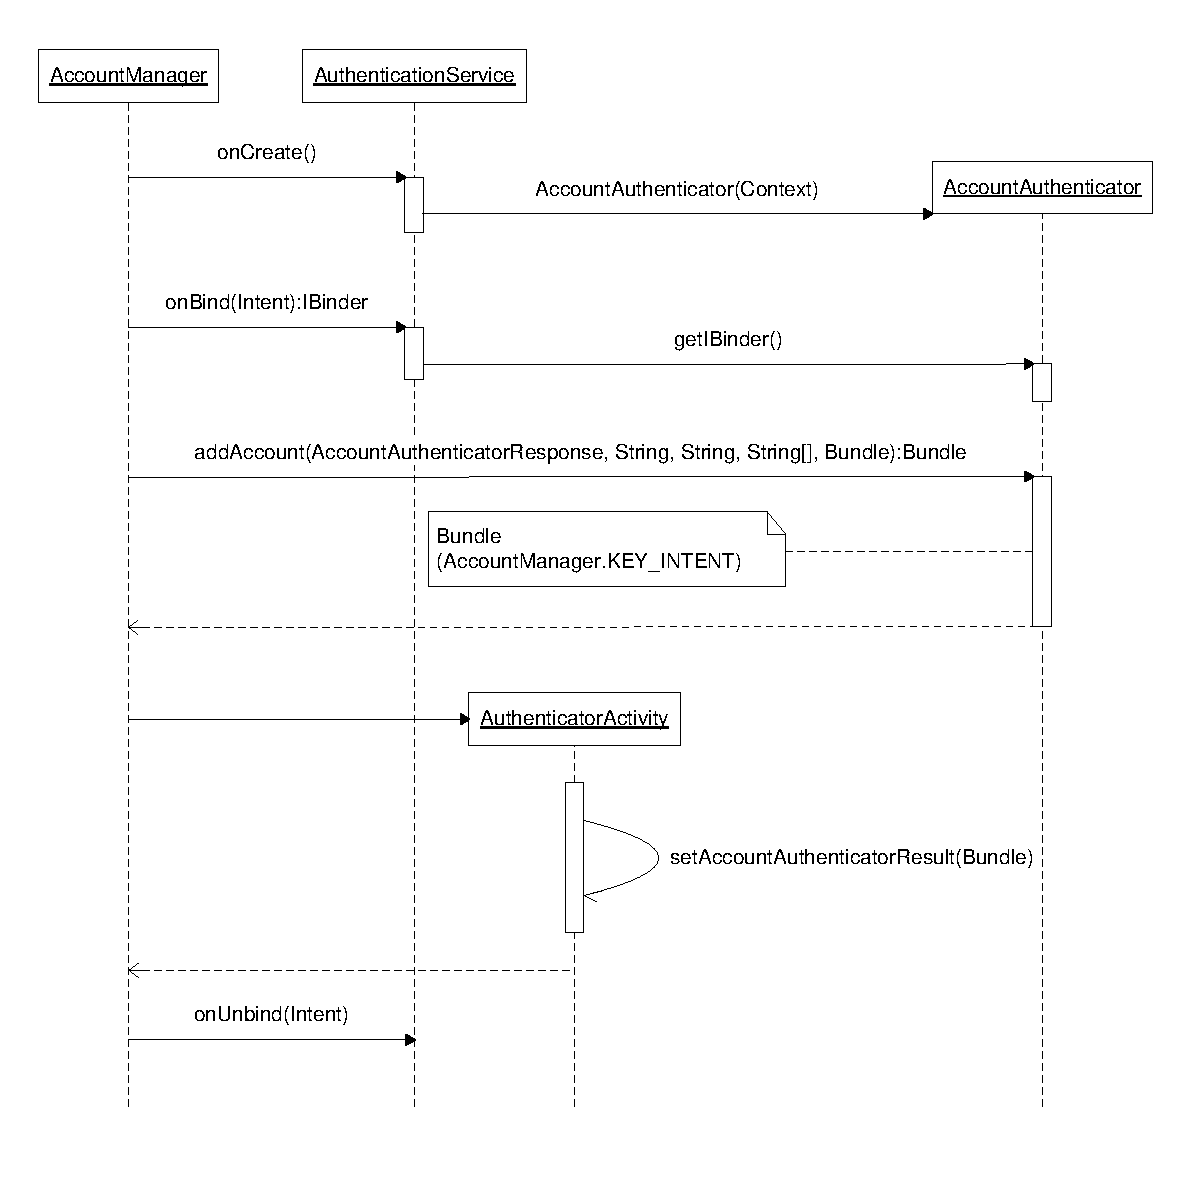
\includegraphics[scale=0.7]{visio/andauth.pdf}
\caption{Sekvenční diagram zobrazující průběh vytvoření účtu}
\label{obr:andauth}
\end{figure}

\begin{figure}
\centering
\begin{minipage}{.5\textwidth}
  \centering
  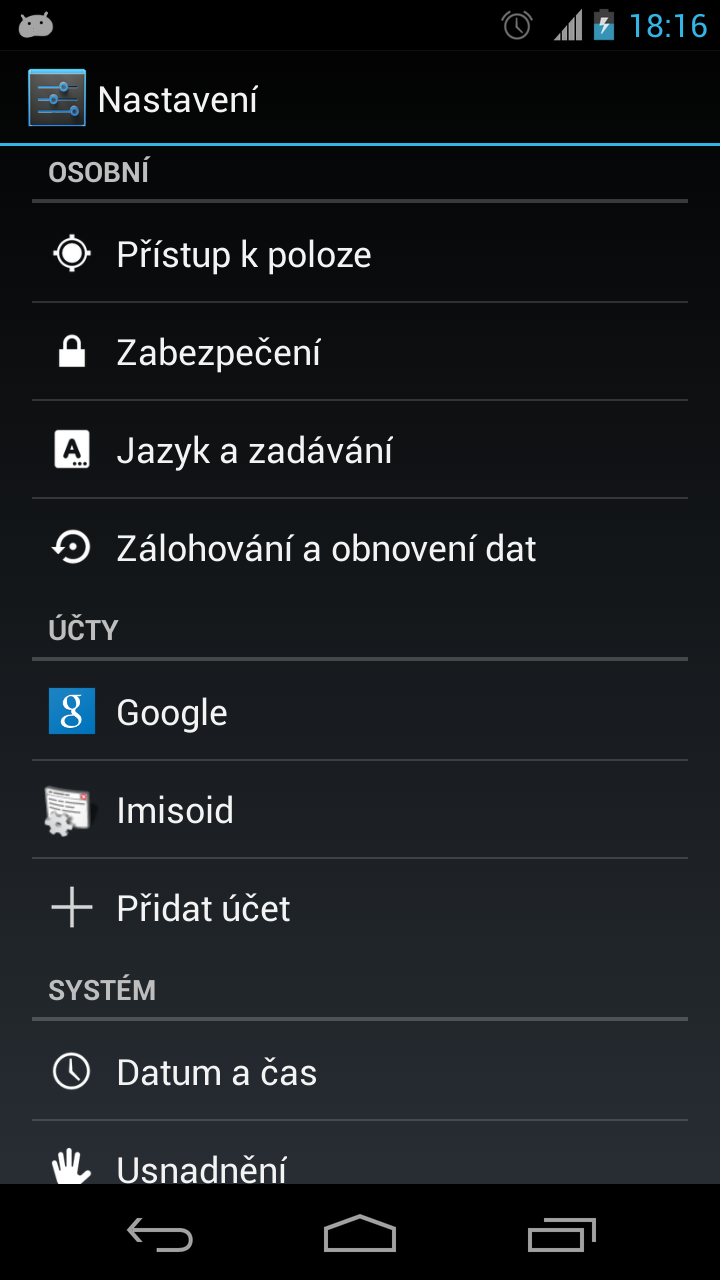
\includegraphics[width=.75\linewidth]{scr/setting.png}
  \captionof{figure}{Nastavení}
  \label{obr:setting}
\end{minipage}%
\begin{minipage}{.5\textwidth}
  \centering
  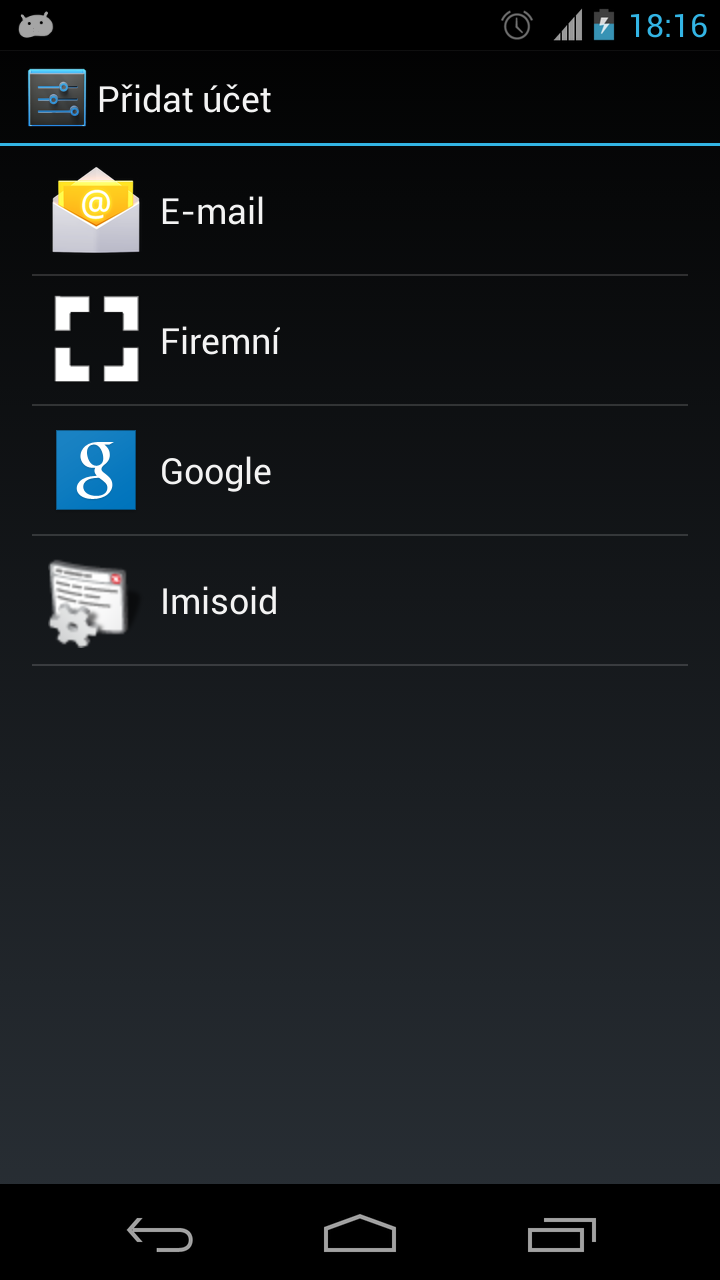
\includegraphics[width=.75\linewidth]{scr/addacc.png}
  \captionof{figure}{Přidání účtu}
  \label{obr:addacc}
\end{minipage}
\end{figure}




\section{Ukládání dat}
Android umožňuje několik způsobů jak persistentně ukládat data aplikace. Programátor by měl vzít v úvahu, zda data mají být soukromá či dostupná i ostatním aplikacím a také velikost těchto dat. 
\subsection*{Sdílené preference} Ukládá primitivní datové typy ve tvaru klíč-hodnota. Slouží k uložení nastavení specifických pro aplikaci. K těmto se přistupuje pomocí \emph{SharedPreferences} rozhraní. Data jsou ukládána persistentně. \\ V aplikaci používám toto úložiště pro nastavení síťového připojení, barevného nastavení pro typy docházkových událostí a další uživatelsky měnitelné hodnoty.\\ \\
Objekty se získávají pomocí příslušné get metody:
\begin{lstlisting}
SharedPreferences settings = PreferenceManager.getDefaultSharedPreferences(context);
int color = settings.getInt("color", defaultColor);
\end{lstlisting}

\noindent
Změny nastavení se provádějí pomocí \emph{SharedPreferences.Editor} rozhraní, které se postará aby data zůstala konsistentní a řídí transkační zpracování.
\begin{lstlisting}
SharedPreferences settings = PreferenceManager.getDefaultSharedPreferences(context);
SharedPreferences.Editor editor = settings.edit();
editor.putInt(("color", userColor);
editor.commit();
\end{lstlisting}

\subsection*{Interní úložiště}
Soubory lze ukládat v interní paměti zařízení. Tyto soubory jsou defaultně přístupné pouze pro aplikace, která je vytvořila a při odinstalování jsou automaticky smazány.
\subsection*{Externí úložiště}
Další možností pro ukládání souborů je externí úložiště (např. SD karta).  Toto úložiště je sdílené a mohou být editována i mimo aplikaci.
\subsection*{SQLite databáze}
Data lze ukládat persistentně pomocí SQLite databáze. Vytvořená databáze je dostupná jakkékoli třídě v aplikaci, ale není přístupná mimo aplikaci, která jí vytořila. SQLite databázi detailněji popisuji v kapitole \ref{sqlite}.

\section{SQLite}
\label{sqlite}
[TODO]je treba resit delku dat napriklad stringu?, dynamic typing

V knihovnách pro Forms aplikace se nachází další kód, který bude nutné přepsat do webové služby.

\section{REST}
RestaTemplates - springframework
\begin{enumerate}
\item REST operace - davkove vs jednotlive
\item REST, tabulka URI, 
\end{enumerate}

\section{Struktura projektu}
(jen ty pouzite)

\section{Manifest + oprávnění}
persmission v manifestu, vypsat a vysvětlit

\section{9png grafika}

\section{GPS}

\section{Zpětná kompatibilita}

\section{Budoucí rozšiřitelnost}

\section{Vytváření grafů}
knihovny, cloudové řešení, vlastní komponenty

\section{Chybové reporty}

\section{Distribuce}

\chapter{Testování}
[TODO testovaci scenare synchronizace]
\section{O čem psát...}
\begin{enumerate}
\item pripraveno webove sluzby na dalsi mobilni platformy
\item cinnost apliakce online/offline
\item flow diagramy pro ruzne cinnosti
\item pristupova prava
\item uspora pesistentni pameti na strane androida
\item chybove reporty a opravy na aplikaci v ostrem prostredi, obrazek + ukazka
\item perioda automatickeho mazani dat
\item datovy model schema
\end{enumerate}

\chapter{Závěr}

\chapter*{Seznam zkratek} 
\addcontentsline{toc}{chapter}{Seznam zkratek}

\begin{list}{}{\setlength{\leftmargin}{30mm}
\setlength{\labelwidth}{30mm} \setlength{\labelsep}{0mm} }
\item[\parbox{30mm}{IMIS}] Integrovaný manažerský informační systém
\item[\parbox{30mm}{ERP}] Enterprise Resource Planning 
\item[\parbox{30mm}{PL/SQL}] Procedural Language/Structured Query Language
%\item[\parbox{30mm}{}]
\end{list}

\appendix
\bibliographystyle{czechiso}
\bibliography{diplomka}
\addcontentsline{toc}{chapter}{Literatura}

\pagestyle{fancy}
\chapter{Uživatelská dokumentace}

\begin{figure}[H]
  \centering
  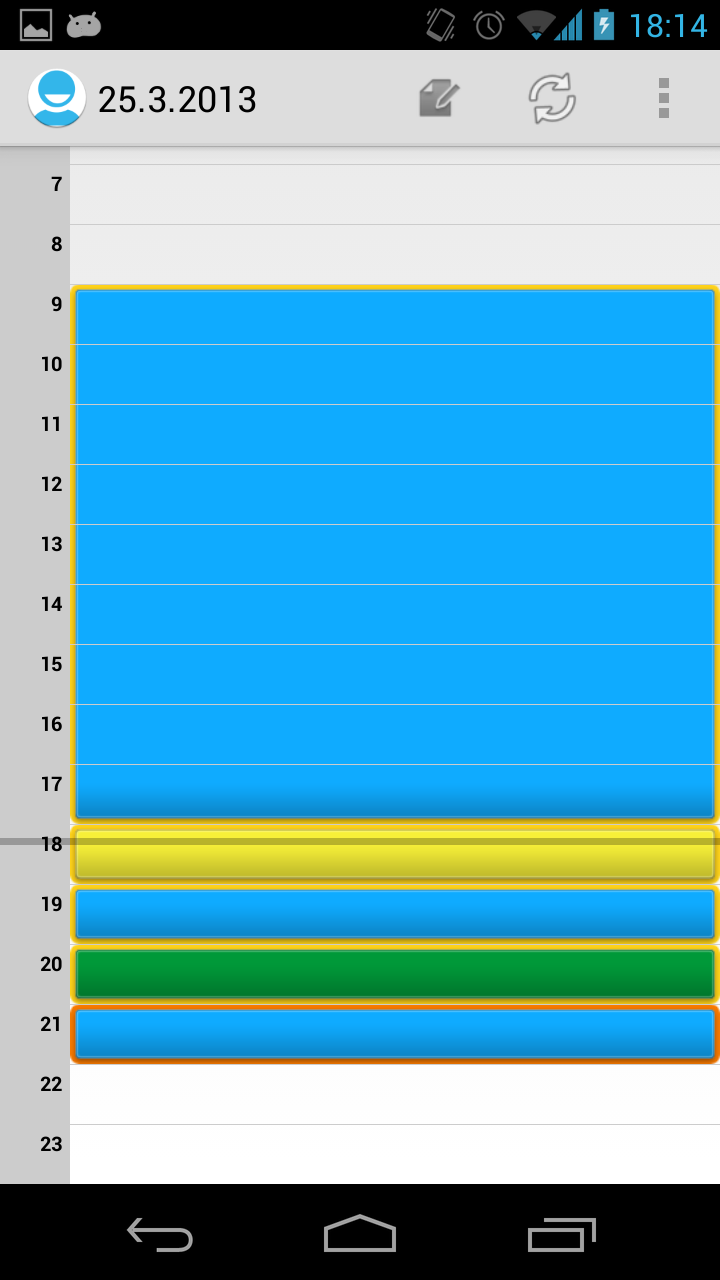
\includegraphics[scale=0.3]{scr/time_doch.png}
  \label{}
\end{figure}

\begin{figure}[H]
  \centering
  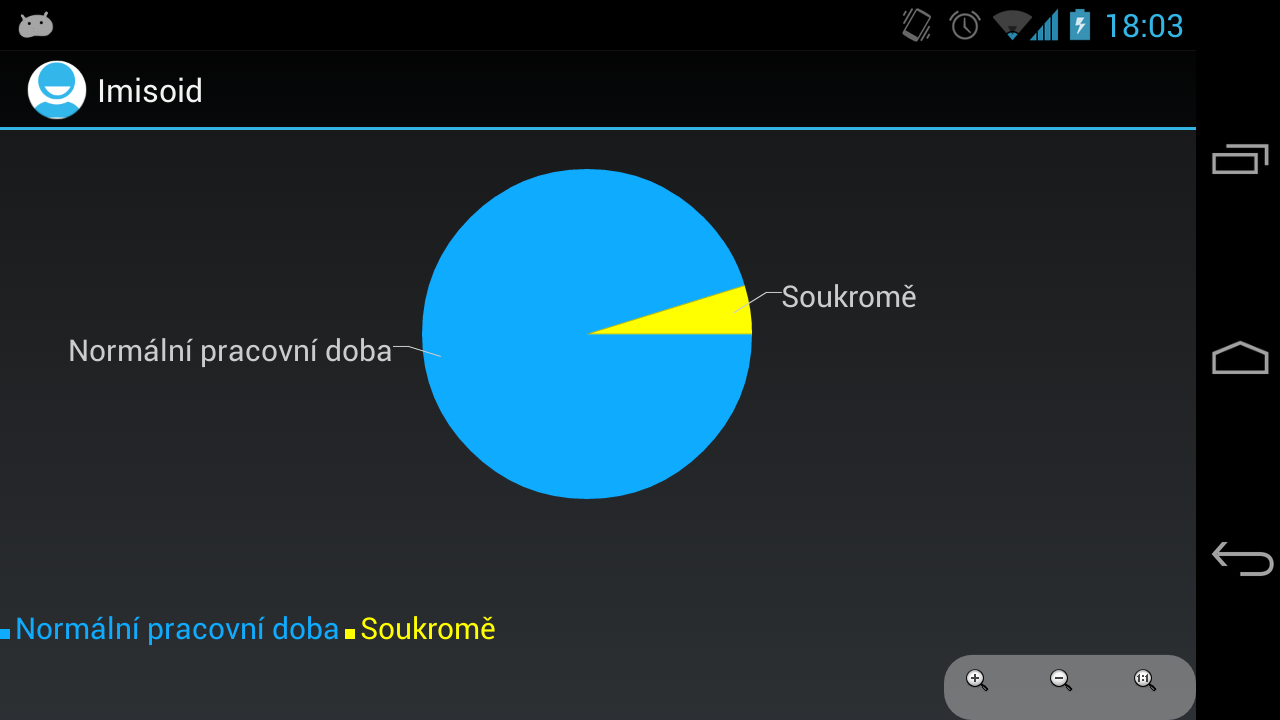
\includegraphics[scale=0.3]{scr/graf_doch.png}
  \label{}
\end{figure}

\begin{figure}[H]
  \centering
  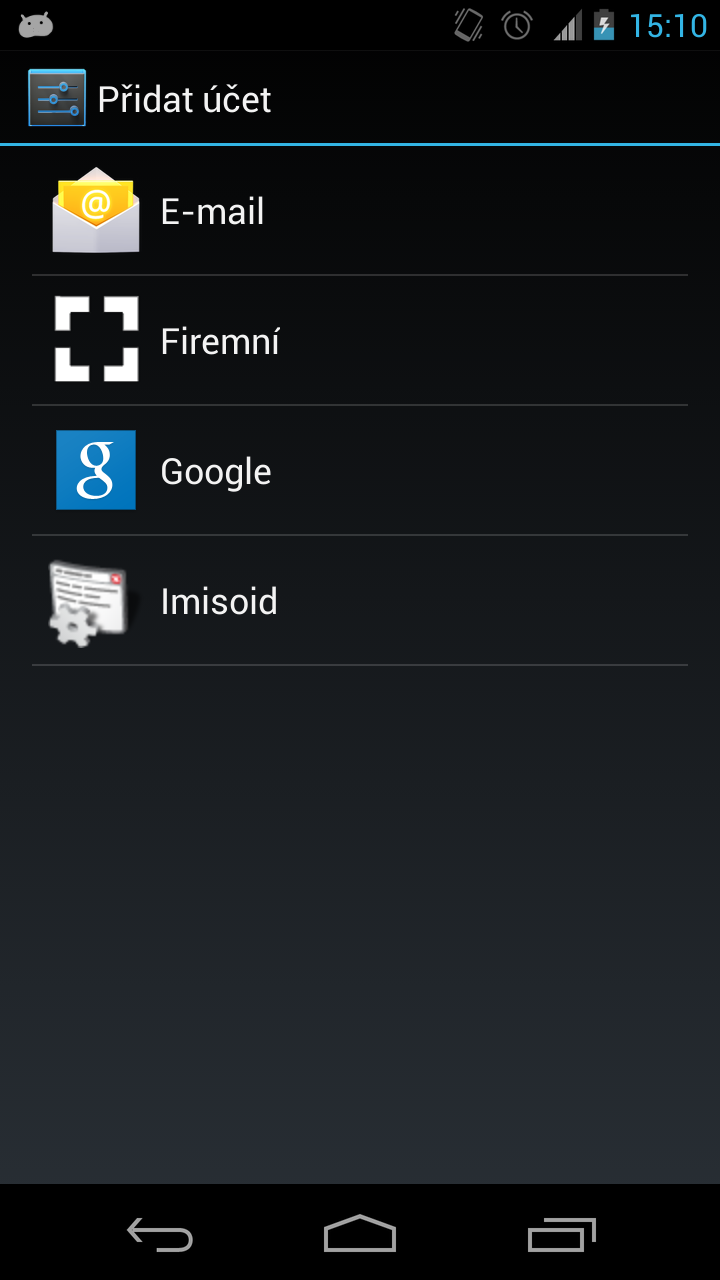
\includegraphics[scale=0.3]{scr/ucet.png}
  \label{}
\end{figure}

\begin{figure}[H]
  \centering
  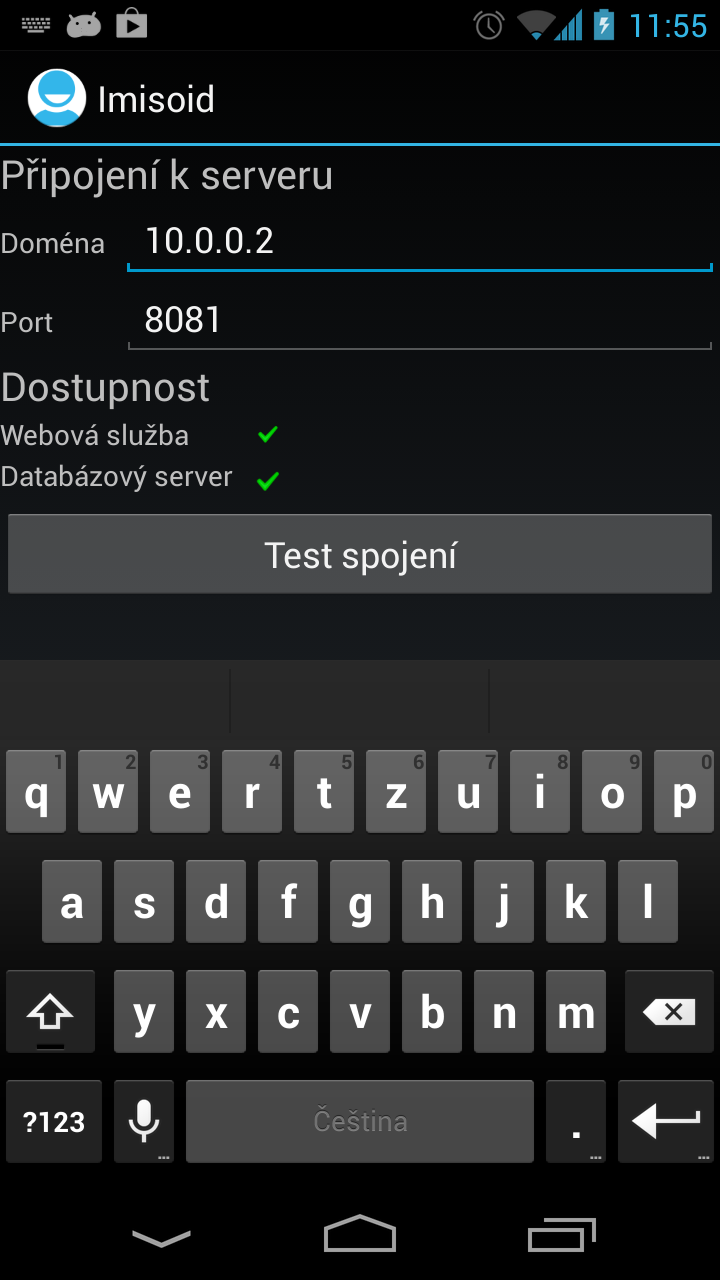
\includegraphics[scale=0.3]{scr/network.png}
  \label{}
\end{figure}

\chapter{Manifest?}

\end{document}
